\documentclass[11pt]{standalone}

\usepackage{helvet}

\usepackage{ifthen}
\usepackage{tikz} 
\usetikzlibrary{shapes.misc}
\usetikzlibrary{arrows,arrows.meta}
\usetikzlibrary{calc,intersections, patterns, math}
\usetikzlibrary{patterns, animations}
\usetikzlibrary{decorations}
\usetikzlibrary{decorations.text}
\usetikzlibrary{decorations.pathmorphing}

\definecolor{pfeil}{RGB}{168,167,167}
\definecolor{petrol}{RGB}{0, 118, 136}
\definecolor{darkgoldenrod}{RGB}{184, 134, 11}
\colorlet{petrol-lighter}{petrol!40}
\colorlet{darkgoldenrod-lighter}{darkgoldenrod!40}

\begin{document}

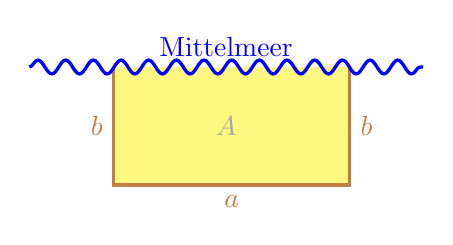
\begin{tikzpicture}[pfeil]

    % \draw[thick, fill=petrol!20, draw=petrol-lighter, rounded corners=2ex, opacity=0.5] (0,0) rectangle ++ (1.5,3.5);
    % \draw[thick, fill=darkgoldenrod!20, draw=darkgoldenrod-lighter, rounded corners=2ex, opacity=0.5] (5,0) rectangle ++ (1.5,3.5);

    \draw[very thick, brown, fill=yellow!50] (0.07,0) -- node[left] {$b$} ++ (0,-1.5) -- node[below] {$a$} ++ (3,0) -- node[right] {$b$} ++ (0,1.5);
	\draw[decorate, decoration={snake}, blue, very thick] (-1,0) -- node[above] {Mittelmeer} (4,0);
	\node at (1.5,-0.75) {$A$};


\end{tikzpicture}

\end{document}
